\subsection{Distributionspolitik} \label{distro}
    Distribution beschreibt die betriebliche Funktion zwischen Hersteller und Verbraucher. Damit beschreibt die
    Distributionspolitik alle Entscheidungen und Maßnahmen auf dem Weg vom Anbieter zum Konsumenten.

    \noindent
    Die Distributionspolitik ist ein maßgebendes Instrument wie an den Kunden herangetreten wird. Die
    Distributionsentscheidungen sind im Regelfall langfristig ausgelegt. Es müssen je nach Produkt komplexe
    Distributionsketten auf- und ausgebaut werden.

    \noindent
    Die Distributionspolitik verfolgt dabei Ökonomische-, Versorgungs- und Psychologische Ziele. Hauptbestandteil der
    Ökonomischen Ziele ist der Erhalt und Ausbau des Betriebs in dem z.B. neue Kundengruppen erschlossen werden. Die
    Versorgungsziele beschäftigen sich unter anderem mit Lieferzuverlässigkeit und Liefergeschwindigkeit. Der dritte
    Bereich, die Psychologischen Ziele beinhalten insbesondere das Auftreten und die Wahrnehmung des Unternehmens.
    (Vgl. \cite{Bruhn2014}, S.\,245-278)

    \noindent
    Distributionswege lassen sich in zwei Arten unterscheiden, den direkten Vertrieb und den indirekten Vertrieb. Bei
    dem direkten Vertrieb übernehmen die Produzenten allein die Gestaltung des Verkaufsprozesses. Das Produkt oder die
    Dienstleistung wird ohne Zwischenhandel an den Konsumenten weitergegeben, z.B. Werksverkauf. Der indirekte Vertrieb
    verzichtet auf einen großen Teil der Distributionsaufgaben und liefert an einen Groß- oder Einzelhändler. Das
    Produkt wird nun entweder vom Händler direkt an den Kunden weitergegeben oder an einen weiteren Händler verkauft.

    \noindent
    Je nach Produkt und Kundengruppe reicht ein Distributionsweg nicht aus, um alle Kunden erreichen zu können. So
    können Unternehmen mit der Mehrwegdistribution über mehrere Absatzwege zeitgleich ihre Kunden erreichen. Eine solche
    Mehrwegdistribution ist mit einem erhöhten Koordinations- und Managementaufwand verbunden ermöglicht es aber
    Unternehmen das Marktpotenzial besser auszuschöpfen und Risiken auszugleichen.

    \noindent
    Auf den verschiedenen Wegen zum Konsumenten werden verschiedene Distributionsorgane angesprochen. Bei einer direkten
    Distribution werden insbesondere unternehmenseigene Distributionsorgane angesprochen. Der indirekte Vertrieb nutzt
    unternehmensfremde Distributionsorgane wie Absatzhelfer (z.B. Spedition) und Absatzmittler (Groß- und Einzelhandel).

    \noindent
    Die Breite der Distributionswegen entscheidet darüber, ob es sich um eine intensive (Universalvertrieb), eine
    selektive (ausgewählte Absatzmittler) oder eine exklusive Distribution (wenige, regulierte Anbieter) handelt.

    \noindent
    Der RinnenRobo soll über eine Mehrwegdistribution unterschiedliche Kundengruppen ansprechen und somit das
    Marktpotenzial bestmöglich nutzen (Siehe folgende Graphik). Per Online-Shop können die Kunden im direkten Vertrieb
    angesprochen werden. Weiter können im B2B Direktvertrieb und auf Messen Unternehmen die als Kunden agieren
    angesprochen werden. Weitere Kunden, wie z.B. den Eigenheimbesitzer können über den indirekten Vertrieb im Baumarkt
    erreicht werden. Die Wahl der Distributionswege lässt auf eine selektive Distribution schließen, welche sich
    besonders durch die Auswahl der Vertriebswege und Anforderungskriterien kennzeichnet. Ein solches Produkt bedarf
    zwar einer gewissen Expertise aber keiner Exklusivität.

     \begin{figure}[ht]
        \centering
        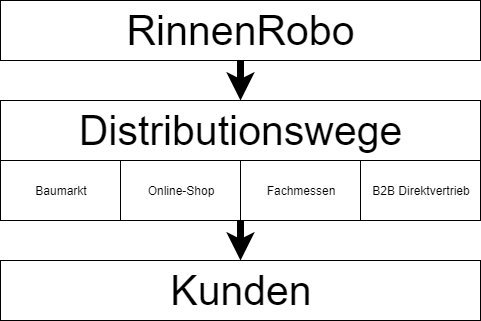
\includegraphics[width = 0.9\textwidth]{Eigene Darstellungen/Distributionswege1.png}

        \caption{Distributionswege (Eigene Dastellung in Anlehnung an Volesungsunterlagen)}
     \end{figure}